\chapter{Contexte}
\paragraph{}
L’Unité de Recherche en Géotechnique (URGéo), dans le cadre de ses activités de recherches et de service à la communauté, dispose d’un ensemble de données géotechniques, géophysiques et géologiques. Le projet consiste à collecter et organiser ces données existantes dans un Système d’Information Géographique (SIG). L’objectif de ces services est donc de concevoir, développer et installer un système de gestion informatisée (base des données) à utiliser dans la gestion de l’archive technique de l’URGéo. Cette unité dispose d'une base de données constituée d’une collection de documents au format PDF (Portable Document Format). Le format PDF est un standard ouvert d'échange de documents électroniques géré par l’ISO (International Organization for Standardization). L’URGéo  souhaite cependant réaliser la migration de cette base vers un système de gestion plus efficace. Elle souhaite aussi pouvoir accéder à cette base via son réseau local.
    \section{Introduction}
        \subsection{Géneral (énoné dans le CDC)}
        \lipsum[1]
        \subsection{Objectif du projet ( énoné dans le CDC)}
        \lipsum[1]
    \section{Réalité des études de sol en Haiti}
    \paragraph{}
    Les données dont dispose l’URGéo proviennent tous d’un ensemble d’études réalisées par ladite instance. Le géologue vérifie non seulement le sol supérieur visible, mais analyse également les couches souterraines en prélevant des échantillons de forage et en creusant des fosses ou des fossés. Les techniciens peuvent effectuer certains tests sur place tandis que d'autres nécessitent une évaluation en laboratoire et peuvent s’avérer être prêts sur des durées longues ou courtes. 
 \par
    Avant d’investir des millions de dollards et des centaines d’heures pour construire un bâtiment, les proprietaires fonciers doivent savoir si le plancher peut supporter le bâtiment en question.Un sous-sol mou et rempli d'air peut conduire à un dépôt plus fort que souhaité, ce qui conduit à des fissures prématurées dans tout le bâtiment.
    \par
    Malgré la valeur que peut coûter de telles études, que ce soit en termes économique et/ou temporel, les caractéristiques d’un sol restent une information essentielle à bien des égards. De ce fait, des études sont réalisées lors de la construction de grandes infrastructures ou de routes. Par exemple : la construction d’un centre départemental d’approvisionnement en intrants pour la direction sanitaire départementale du sud’est. 
    \cite{realisationGeotechsol}
    
        \subsection{Les données géotechniques en Haiti}
       \paragraph{}
       Diverses instances séparées détiennent des données recueillies au cours de leurs études respectives. En effet, la sensibilité et l’importance de ces dernières exigent l’existence de responsables dédiés à cette fin. Ainsi, lorsqu’un particulier a besoin de faire des études de sols, il fait appel à des instances clés capable de les prendre en charge. 
       \paragraph{}
        Parmi celles accessibles dans le pays, les plus contactées restent :
        \begin{itemize}
            \item \textbf{URGéo}
        L'Unité de Recherche en Géosciences a pour mission de mener des recherches dans les
        domaines des géosciences où elle a les capacités pour le faire.
        Cela implique une bonne compréhension des différentes problématiques liés au sol et
        au sous-sol et la proposition de moyens de mitigations adaptées à la réalité haïtienne.
        \cite{mission_urgeo}
        \\
        Pour le moment, l’URGéo constitue l’une des rares unités de recherches dédiée aux
        géosciences dans le pays. 
        Ces chercheurs prennent part à de grandes réunions savantes et scientifiques en
        Amérique du Nord, en Europe et dans les Caraïbes.
        \cite{urgeo_nouvelliste}
            \item \textbf{BME}
        Le Bureau des Mines et de l’Energie (BME) est un organisme autonome créé en 
        1986 fonctionnant sous la tutelle du Ministre des Travaux Publics, Transports 
        et Communications (MTPTC). Sa mission principale est de promouvoir la recherche
        et l'exploitation des ressources minérales et énergétiques d'Haíti ainsi que les 
        techniques appropriées y relative.
            \item \textbf{SICOD}
        La  Société d’Ingénierie Constructions et d’Orientations Diverses (SICOD),
         fondée en 2011, est une société haïtienne en noms collectifs qui évolue dans les domaines d’ingénierie géotechnique et de constructions.
         Il s'adonnent aux prélèvements des données des essais de laboratoire, des interprétations systématiques et aux recommandations techniques. 
         Ils apportent leur support technique aux maîtres d'ouvrages dans la réalisation de leur chantier tout en observant les critères techniques de l'art.
            \item \textbf{LNBTP}
        Le LNBTP est une institution publique à gestion autonome chargée du contrôle de la qualité des infrastructures en construction dans le pays. Il s'occupe 
        aussi des études géotechniques, des recherches appliquées sur les matériaux de construction et de la promotion des normes en matière de génie civil.
            \item \textbf{Géothechsol}
        Géothechsol est un Bureau d’Etudes en Ingénierie Géotechnique et Environnemental ainsi qu’en formulation de béton et ses essais mécaniques et physiques,
         qui s’est fixé pour objectif de vous apporter une réponse sérieuse et de qualité, adaptée à vos besoins dans le respect de vos contraintes.
         Ce bureau axe ses travaux sur les essais géotechniques et des sondages.
        \end{itemize}
        
        
        \subsection{Leurs réalisations}
        En général ces entreprises s'impliquent dans la construction et la recherche. 
        Leur travail consiste à effectuer une reconnaissance/étude géotechnique des sites et des échantillons  sont sélectionnés pour des analyses au
        laboratoire.
        \par
        Depuis plusieurs années ils se sont fait remarquer, notamment dans
         l'étude des sols avant la construction de grands bâtiments. Ils sont aussi impliqués dans la réalisation des ponts et des routes sur le territoire
          haitiens. Cependant la concurrence est rude car des firmes étrangères sont parfois appelées. 
     
     
     
          \section{Les BDD géotechniques dans le monde}
        Haïti n’est pas le seul pays à se préoccuper de la gestion de ces données sensibles sur son territoire. Par ailleurs, des SIG ont vu le jour partout à travers le monde.
        \subsection{Dans les Caraïbes}
        \paragraph{Elaboration d'une Base de Données Géotechniques
        sur 1'Ile de Cayenne: }
        Elle a été élaborée dans le cadre d'une convention passée entre la
        Région de Guyane et le BRGM en 2001.
        \cite{Cayenne}
         L'objectif était de constituer une base de données renseignée regroupant tous les points (sondages, essais
        in situ ou en laboratoire) améliorant la connaissance des caractéristiques géomécaniques des
        formations d'une zone de projet. Cela permettra de mieux appréhender les types de problèmes
        spécifiques au site, et donc de mieux dimensionner les campagnes de reconnaissance
        géotechniques, aussi bien sur le plan technique que financier.
       \paragraph{ Principes de fonctionnement de l'application ACCESS: }
       Une base de données est un ensemble d'informations associées à un sujet particulier.
        Microsoft Access, permet de gérer toutes les informations en respectant les relations définies
        par le modèle conceptuel des données, à l'aide d'un fichier unique de base de données. Dans
        ce fichier, les données sont réparties entre plusieurs contenants appelés tables. [...]
        Pour permettre la consultation de ces données, BD-GTC contient des formulaires qui
        permettent de consulter, d'ajouter et de mettre à jour les données des tables. L'ensemble de ces
        formulaires constitue l'application BD - GTC.
        \cite{Cayenne}

        \subsection{En Amérique}
        \paragraph{Conception d'une architecture d'information géotechnique à l'aide de services Web}
        Cette architecture d'information a été implémentée à Los Angeles afin de permettre les échanges 
        d'informations géotechniques accessibles pour tous. Les avantages apportés par une telle 
        application pourraient tant se sentir pour des études concernant les risques sismiques que pour 
        une meilleure approche lors des estimations effectuées par des compagnies d'assurance. 
        \cite{zimmermann2003design}
        \paragraph{Base de données géoscientifique régionale pour le projet de la moraine d'Oak Ridges}
        Une base de données géoscientifiques est élaborée dans le but d’aider à la finalisation de la 
        cartographie des dépôts en surface et en subsurface dans la région de la moraine d’Oak 
        Ridges. Elle se compose de trois éléments : a) une base de données relationnelles, 
        b) des couches de données intégrées à un système d’information géographique (SIG) 
        et c) des fichiers plats.
        \cite{russell1996regional}
        \paragraph{Intérêt des utilisateurs finaux pour les systèmes de gestion des données géotechniques}
        La centralisation des données facilite la tâche des utilisateurs qui pourront ainsi acccéder à ces
        données de façon continue et plus efficace.
        \cite{Turner2008}

        \subsection{En Europe}
        % 4 Subsurface data base in geoenvironmental engineering
        \cite{antoljak2012subsurface}
       
        \lipsum[1]
        \subsection{La Nouvelle-Zélande}
        \paragraph{CGD}
        La base de données géotechnique de Canterbury (CGD) est une base de données en ligne qui a été développée pour
        la reconstruction de Christchurch à la suite du tremblement de terre de Canterbury 2010-2011 (CES). Il
        a été conçu comme un référentiel consultable pour le partage d'informations géotechniques existantes et nouvelles
        ainsi que des applications géotechniques de soutien pour les autorisations de construction et de ressources. En mars
        2015, la base de données contient plus de 18000 enregistrements d'essais de pénétration de cône, 4000 forages, 1000
        piézomètres accompagnés de registres de surveillance des eaux souterraines, 6000 enregistrements de tests de laboratoire
        plus d'autres données. Ces données peuvent également être utilisées à des fins plus stratégiques telles que l'aide à la
        relèvement en cas de futures catastrophes naturelles, accroissement de la résilience d'autres régions de la Nouvelle-Zélande,
        modélisation des sinistres catastrophiques et information des processus réglementaires. La vaste base de données géotechnique
        combinée à d'autres ensembles de données permet un examen et une modélisation approfondis du terrain
        et la performance de l'infrastructure construite. Les leçons tirées de ces analyses peuvent être appliquées
        améliorer la résilience et également utilisé pour éclairer les décisions de politique réglementaire dans d'autres domaines de
        Zélande.
        \par
        Le CGD a été conçu comme un référentiel consultable pour les informations géotechniques existantes et nouvelles
        ainsi que des applications géotechniques de soutien pour les autorisations de construction et de ressources. Tandis que le
        les données sont principalement utilisées pour la conception géotechnique de l'amélioration du sol, la fondation du bâtiment
        réparations, fondations de nouveaux bâtiments et conception géotechnique pour les réparations d'infrastructures, il peut
        également être utilisé à des fins plus stratégiques telles que l'aide à la récupération pour de futurs
        catastrophes naturelles, augmentation de la résilience d'autres régions de la Nouvelle-Zélande, modélisation des
        informer les processus réglementaires.
        \cite{cgd}

       
        \begin{figure}[t]
        \centering
        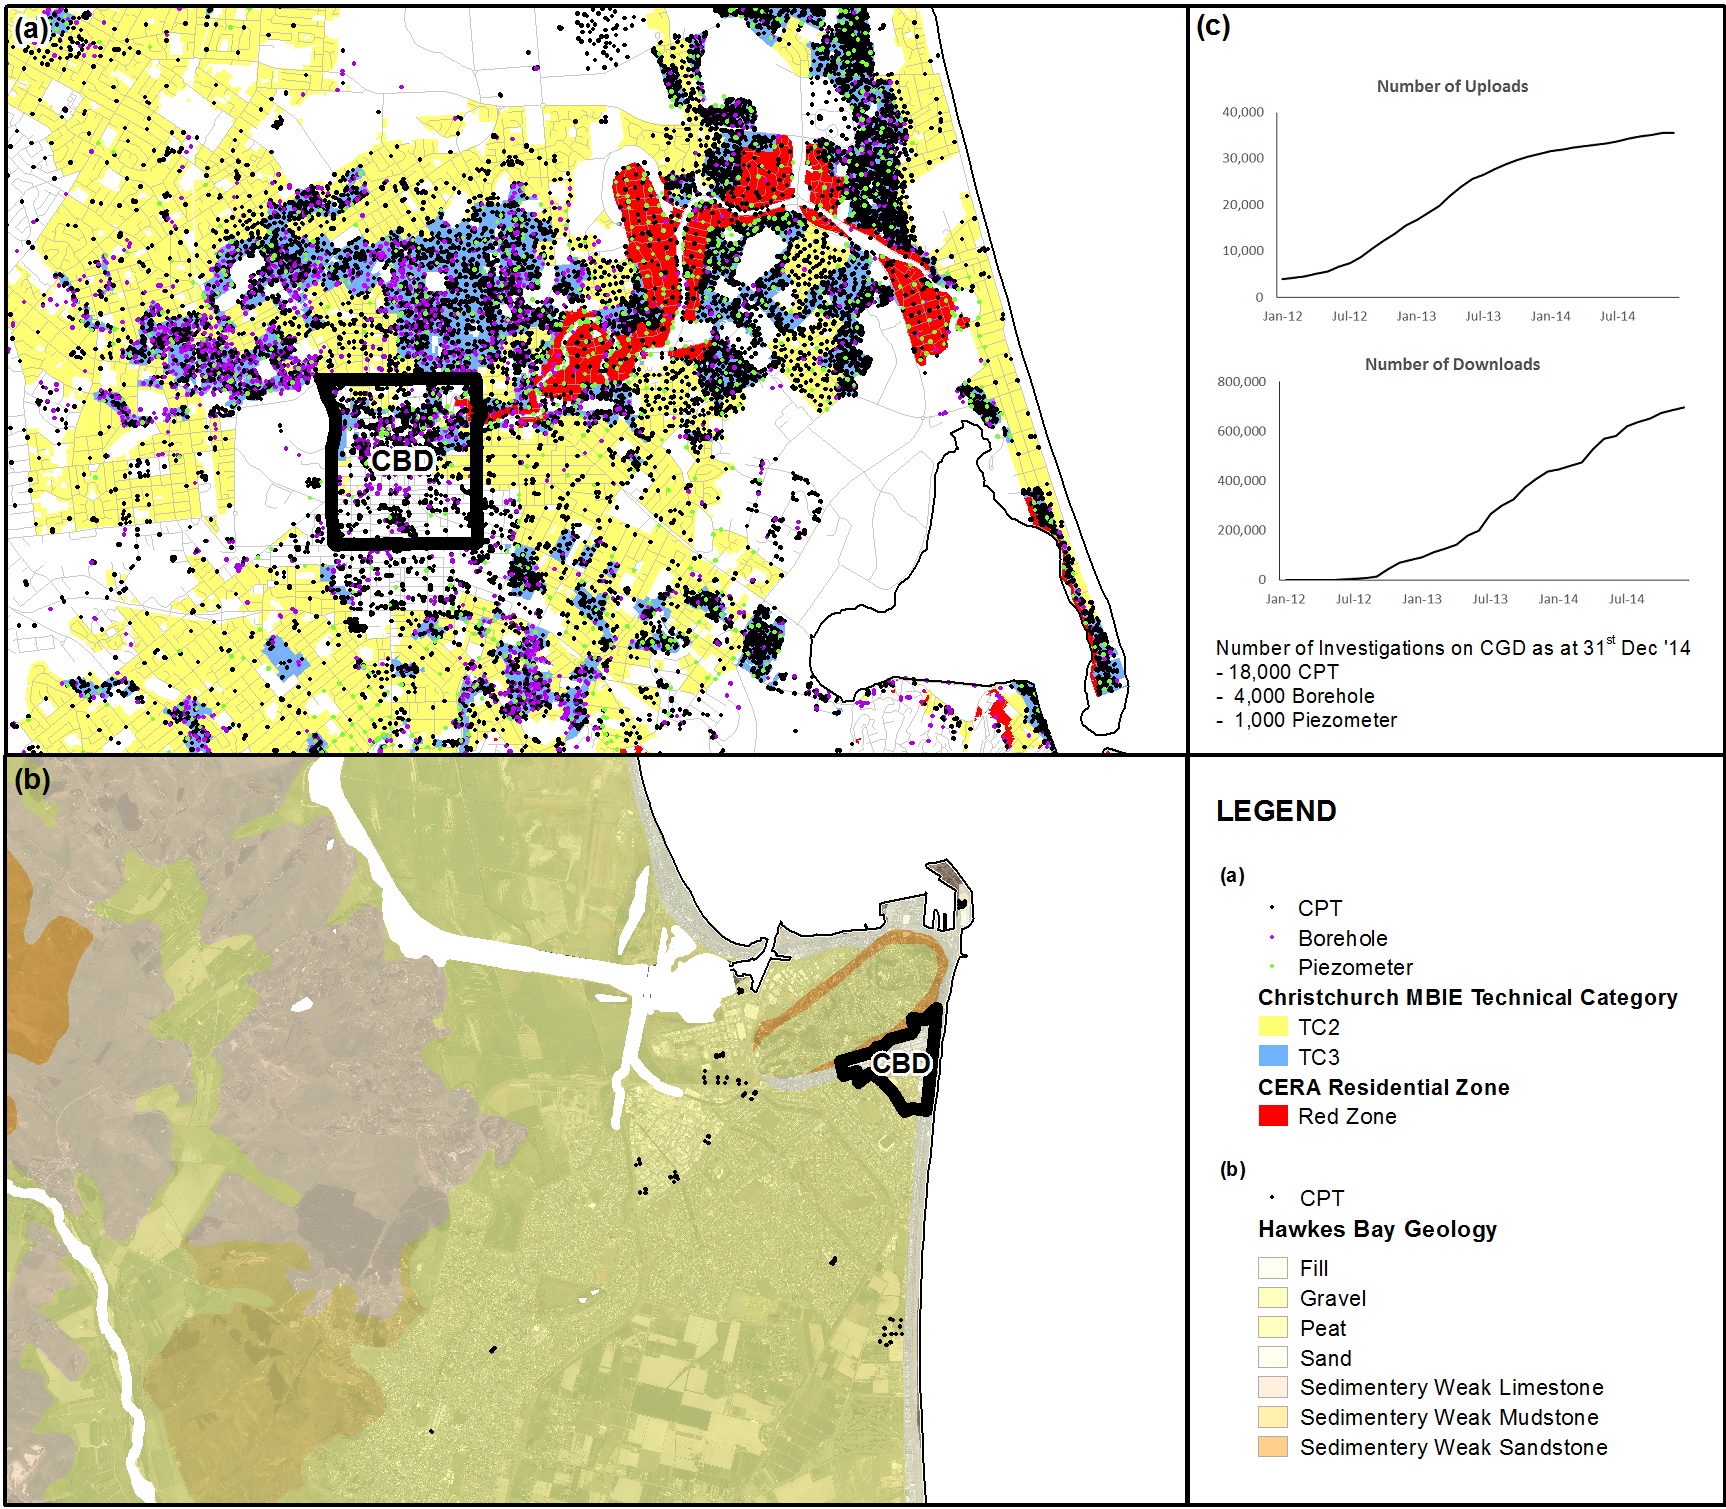
\includegraphics[width=1\textwidth]{cgd.png}
        \label{image-cdg}
        \caption{Visualisation des résultats de la base de données de Canterbury.}
        \end{figure}
        %Management of geotechnical data and processes
        \subsection{En Asie}
        % \par
        %  EGU2016-2503Poster,
        %  5 db development in bangkok
         \paragraph{}

         \subsection{En Afrique}
            \paragraph{Base de données géologiques et géotechniques orientée vers la cartographie géotechnique: Application à la ville de Tunis (Tunisie)}
            Il s'agit de la méthodologie mise au point pour Ia conception et la realisation d'une base de donnees géologiques et géotechniques.
            Différents types ou données  sont collectées, leur structure et leur stokage sous forme de fichiers inddpendants. Est également
            developpée la manipulation de la base en particulier la consultation de TUNIS-DATA-BANK.
            \par
            Le modèle choisi nous a permis, après une analyse
pré1iminaire très importante, une description globale et
totale de toutes les données géologiques et géotechniques collectées sur le site de Tunis (TUNISIE). I1
assure, de plus, une indépendance physique et logique,un partage des données (une même donnée accessible  par plusieurs programmes), une non redondance des données, une non codification des
données géologiques, une grande facilité des relations
entre fichiers indépendants, une intégrité (validité)
totale des données. S'y ajoutent une souplesse remarquable d'interrogation de TUNIS-DATA-BANK
assurée par l'emploi d'un langage d'interrogation spécifique et l'utilisation des operateurs et des connecteurs
logiques, une automatisation totale des taches de la
phase de la manipulation de la base de données et une
sbcurité totale des fichiers.
\cite{tunis}
 % STAL9781607500315-3360
%         Ce Rapport Général passe en revue les thèmes de la Gestion des Données et des Procédés de Géotechnique sur la base des documents
% soumis à la 17e Congrès International de Mécanique des Sols et de la Géotechnique, à Alexandrie, en Égypte. Les contributeurs
% conviennent que les normes de données sont nécessaires pour permettre l'interchangeabilité et de partage des données géotechniques.
% Ainsi, l'évolution de la représentation des données en utilisant XML sont décrites qui permettra à la World Wide Web à devenir un
% référentiel international pour l'information géo-ingénierie. XML fournit la flexibilité nécessaire pour la représentation des données
% hétérogènes obtenus à partir de la surveillance sur le terrain. Systèmes d'information géographique (SIG) offrent de grandes
% opportunités pour les ingénieurs en géotechnique, en particulier pour le stockage de grandes quantités de données de forage. La
% nécessité pour le traitement des incertitudes et de gestion des risques dans l'ingénierie géotechnique est mis en évidence. Le partage
% des risques devrait faire en sorte que chaque risque est assumé par la partie la mieux à même de contrôler, compte tenu de leur
% compétence technique et les engagements contractuels. Mesures d'atténuation des risques doivent être mis en place lorsque le niveau
% de risque est élevé. Event Tree Analysis constitue un bon moyen d'évaluer les niveaux de risque, et peuvent intégrer les compétences
% de différentes disciplines. De plus grandes quantités de données d'enquête sur site permettra de réduire la probabilité de sous-ou sur-
% conception des ouvrages géotechniques, bien que mai est un point optimal au-delà de laquelle des données fourniront amélioration
% limitée. Le degré d'incertitude dans l'ingénierie géotechnique est évident à partir d'un exercice d'étalonnage de la réponse sismique du
% site d'analyse a montré que les variations d'un maximum de 4100% entre les équipes participantes, les évaluations de la même entrée
% de données. Destranslate exemples et études de cas sont décrits dans les domaines d'application des pentes et les glissements de terrain et
% l'évaluation des aléas sismiques.
        % \cite{Toll}
    \section{Comparaison entre les outils déjà implémentés}
    \paragraph{}
    L’implémentation de tous ces SIG créés par des organismes internationaux résulte à des données considérées 
    comme étant le système d’archivage officiel dans leur domaine de spécialité.
     Le rythme de migration de ces données dans le SIG Web connait une croissance exponentielle. 
     Un important volume de contributions venant combler les lacunes au plan mondial est aujourd’hui publié en ligne.
      La couverture des informations géographiques à l’échelle planétaire est continue : elle constitue le SIG du monde.
    \section{Gestion actuelle des données géothechniques en Haïti}
    Jusqu’à date, chaque instance détient ses données propres, dans un format qu’elle est seule habilité à définir. Beaucoup d’entre elles sont encore a l’ère du papier. D’autre utilisent comme base de données des fichiers Excel. Enfin une infirme partie a construit une base donnée dediée. Cependant toutes ces informations utiles  se trouvent éparpillées. Cette distribution n’est pas la meilleure quand il s’agit d’annalyser ou de concevoir des modeles statitiques  visant à optimiser les études géotechniques.

    \subsection{Apport de ce projet}
    La gestion informatique du laboratoire est aujourd’hui devenue incontournable pour répondre aux contraintes normatives, techniques et commerciales d’une démarche d’assurance qualité. Dans cet esprit, la mise en œuvre d’une base de données documentaire et cartographique permettant la gestion intégrée des essais et du système est une condition nécessaire à l’atteinte des objectifs de qualité. Celle-ci, intégrée à un portail web, permettrait entre autres de renforcer la communication commerciale et l’image de l’URGéo en tant qu’unité de recherche et de service.
De plus en établissant une base de donnée géotechnique centralisée, il y aura une entreprise phare lorsqu’une entité quelconque (université, ingénieur,...) s’interesse au profil géotechique d’Haïti.
 \par 
    Avec une base de données géoenvironnementale correctement mise en œuvre, 
    toutes les données souterraines sont centralisées et consolidées afin que 
    la recherche et l'interrogation des données deviennent intuitives et 
    transparentes, ainsi que la création de rapports et la publication.
        %penser aux objectifs